% !TeX root = mos-en.tex

%%%%%%%%%%%%%%%%%%%%%%%%%%%%%%%%%%%%%%%%%%%%%%%%%%%%%%%%%%%%%%%%

\refstepcounter{problem}  % 41. The locomotive problem

%%%%%%%%%%%%%%%%%%%%%%%%%%%%%%%%%%%%%%%%%%%%%%%%%%%%%%%%%%%%%%%%

\newpage

\begin{prob}{The little end of the stick}
A large number of glass rods each of length $1$ are broken into two pieces each. The breaking point is uniformly distributed along the lengths of the rods.

\que{1} What is the expectation of the length of the \emph{smaller} piece?

\que{2} What is the expectation of the ratio of the length of the smaller piece to the length of the larger piece?
\end{prob}

\solution{}

\ans{1} The probability that the break is on the left half of a rod is $1/2$ as is the probability that it is on the right half.
The smaller piece is on the same side as the break so the expectation of its position is halfway between the middle and the end:
\[
E(\textsf{length of smaller piece}) = \frac{1}{2}\cdot\frac{1}{2}=\frac{1}{4}\,.
\]

\ans{2} Without loss of generality assume that the break occurred in the right half of the rod (Figure~\ref{f.stick}). The ratio of the smaller piece to the larger piece is $(1-x)/x$ and a normalization constant (page~\pageref{p.normal}) must be used because the expectation is computed over 
$(1/2,1)$,
half the range of $x$:
\begin{eqn}
E(\textsf{ratio of smaller to larger})&=&\left(\frac{1}{1-(1/2)}\right)\int_{\textstyle\frac{1}{2}}^1 \frac{1-x}{x} \,dx\\
&=& 2\int_{\textstyle\frac{1}{2}}^1 \left(\frac{1}{x} -1\right) \,dx \\
&=& 2 (\ln |x| - x)\left|^{\stackrel{\scriptstyle 1}{\rule{0pt}{4pt}}}_{\textstyle\frac{1}{2}} \right. = 2(0-1 -\ln \textstyle\frac{1}{2}  + \textstyle\frac{1}{2})\approx 0.3863\,.
\end{eqn}%
\begin{figure}[tb]
\begin{center}
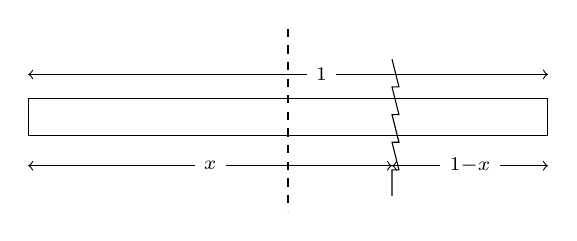
\begin{tikzpicture}[scale=1.1]
\draw (0,0) -- ++(6,0) -- ++(0,12pt) -- ++(-6,0) -- cycle;
\draw[<->] (0,20pt) --
  node[fill=white,xshift=12pt] {$\scriptstyle 1$} ++(6,0);
\draw[decorate,decoration=saw] (4.2,25pt) -- +(0,-45pt);
\draw[thick,dashed] (3,35pt) -- +(0,-60pt);
\draw[<->] (0,-10pt) --
  node[fill=white] {$\scriptstyle x$} (4.2,-10pt);
\draw[<->] (4.2,-10pt) --
  node[fill=white] {$\scriptstyle 1-x$} (6,-10pt);
\end{tikzpicture}
\end{center}
\caption{Breaking a stick into two pieces}\label{f.stick}
\end{figure}


\sml{}
\begin{verbatim}
Expectation of length of smaller = 0.2500
Average length of smaller        = 0.2490
Expectation of smaller/larger    = 0.3863
Average smaller/larger           = 0.3845
\end{verbatim}

%%%%%%%%%%%%%%%%%%%%%%%%%%%%%%%%%%%%%%%%%%%%%%%%%%%%%%%%%%%%%%%%


\begin{prob}{The broken bar\annotate{D}}

A large number of glass rods of length $1$ are broken in two places (\ref{f.break1}).

\que{1} What is the expectation of the length of the shortest piece?

\que{2} What is the expectation of the length of the longest piece?

\textbf{Hint:} $x,y$ are independent random variables with a uniform distribution from $(0,1)$. Each pair $(x,y)$ can be represented as a point in the unit square $(0,1)\times (0,1)$ (\ref{f.break2}). From the Figure can you compute is the probability that $(x,y) < (.5,.25)$?

\textbf{Hint:} For \quenc{1} assume that left piece is the shortest one and for \quenc{2} assume that the left piece is the longest one.
\begin{figure}[tb]
\begin{center}
\begin{subfigure}{.4\textwidth}
\begin{tikzpicture}[scale=.8]
\draw (0,0) node[below left] {$0$} --
  ++(6,0) node[below right] {$1$} --
  ++(0,12pt) -- ++(-6,0) -- cycle;
\draw[<->] (0,20pt) --
  node[fill=white] {$\scriptstyle 1$} ++(6,0);
\draw[decorate,decoration=saw] (1.8,25pt) -- +(0,-45pt);
\draw[decorate,decoration=saw] (4.7,25pt) -- +(0,-45pt);
\node[below left] at (1.8,0) {$x$};
\node[below left] at (4.7,0) {$y$};
\path (0,-3.5) rectangle +(0,3.5);
\end{tikzpicture}
\caption{Break a rod into two pieces\hspace{6em}\mbox{}}\label{f.break1}
\end{subfigure}
\hspace{3em}
\begin{subfigure}{.4\textwidth}
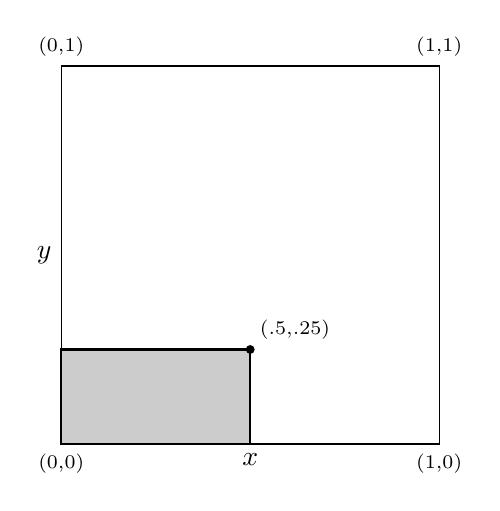
\begin{tikzpicture}[scale=.8]
\draw (-3,-3) rectangle +(6,6);
\draw[thick,fill=white!80!black] (-3,-3) -- ++(0,1.5) -- 
  ++(3,0) -- ++(0,-1.5) -- cycle;
\path (-3,-3) node[below] {$\scriptstyle (0,0)$} --
  node[below] {$x$} (3,-3)
  node[below] {$\scriptstyle (1,0)$};
\path (-3,-3) -- node[left] {$y$} (-3,3)
  node[above] {$\scriptstyle (0,1)$};
\node[above] at (3,3) {$\scriptstyle (1,1)$};
\fill (0,-1.5) circle [radius=2pt]
  node[above right] {$\scriptstyle (.5,.25)$};
\end{tikzpicture}
\caption{Representation of the lengths in the unit square}\label{f.break2}
\end{subfigure}
\end{center}
\end{figure}
\end{prob}

\solution{}

\ans{1} Without loss of generality assume that the left piece of length $x$ is the shortest. Then $x<y-x$ and $x < 1-y$, from which we have $2x<y$ and $x+y<1$.

\ref{f.shaded1} shows the lines $y=2x$ (red) and $y=1-x$ (blue).  For the inequalities to be true, $(x,y)$ must be in the shaded region left of the two lines. The point of intersection $(1/2,2/3)$ can be computed by solving the two equations.

The expectation is computed by integrating the product of $x$ and the difference between the two lines. The normalization constant is the area of the square divided by the area of the shaded region:
\begin{eqn}
E(x)&=& \frac{1}{1/6}\int_{0}^{1/3} x [(1-x)-2x]\,dx\\
&=&6\int_{0}^{1/3} (x -3x^2)\,dx\\
&=&6\left. \left(\frac{x^2}{2}-x^3\right)\right|_0^{1/3}=\disfrac{2}{18}\approx 0.1111\,.
\end{eqn}%

\begin{figure}[tb]
\begin{center}
\begin{subfigure}{.46\textwidth}
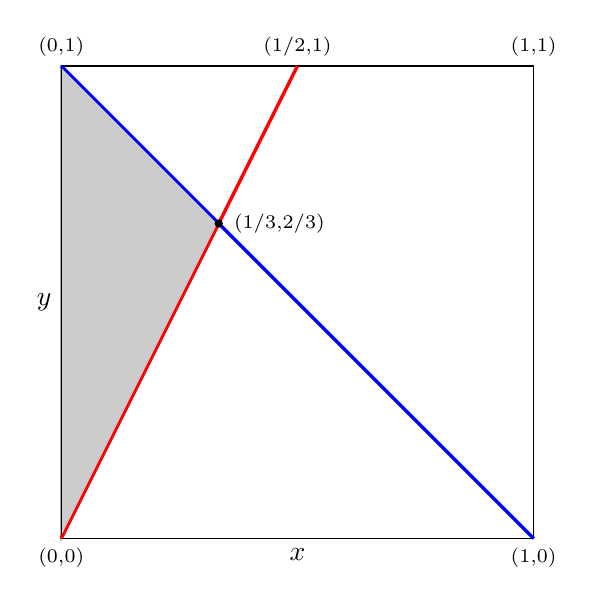
\begin{tikzpicture}[scale=1]
\draw (-3,-3) rectangle +(6,6);
\path (-3,-3) node[below] {$\scriptstyle (0,0)$} --
  node[below] {$x$} (3,-3)
  node[below] {$\scriptstyle (1,0)$};
\path (-3,-3) -- node[left] {$y$} (-3,3)
  node[above] {$\scriptstyle (0,1)$};
\draw[red,very thick]  (-3,-3) -- (0,3);
\draw[blue,very thick] (-3,3)  -- (3,-3);
\coordinate (P) at (-1,1);
\draw[fill=white!80!black] (-3,-3) -- (P) -- 
  (-3,3) -- cycle;
\draw[red,thick]  (-3,-3) -- (0,3);
\draw[blue,thick] (-3,3)  -- (3,-3);
\fill (P) circle[radius=1.5pt]
  node[right,xshift=2pt] {$\scriptstyle (1/3,2/3)$};
%\draw[thick,dotted] (-3,-3) -- (3,3);
\node[above] at(0,3) {$\scriptstyle (1/2,1)$};
\node[above] at(3,3) {$\scriptstyle (1,1)$};
\end{tikzpicture}
\caption{Shaded area for shortest bar}\label{f.shaded1}
\end{subfigure}
\hspace{1em}
\begin{subfigure}{.46\textwidth}
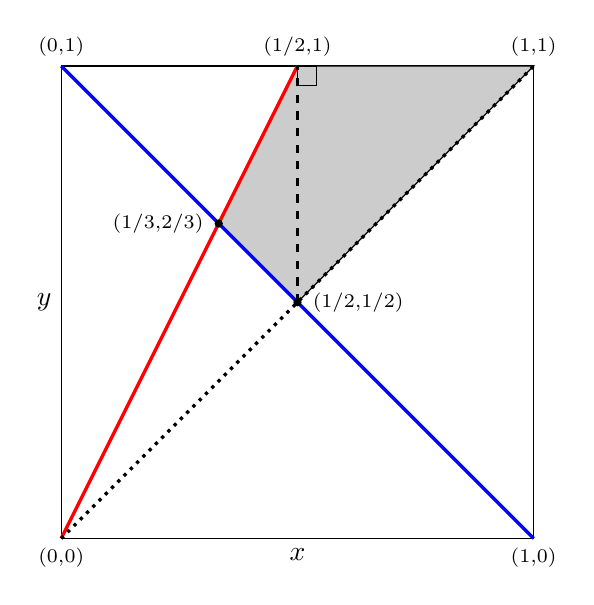
\begin{tikzpicture}[scale=1]
\draw (-3,-3) rectangle +(6,6);
\path (-3,-3) node[below] {$\scriptstyle (0,0)$} --
  node[below] {$x$} (3,-3)
  node[below] {$\scriptstyle (1,0)$};
\path (-3,-3) -- node[left] {$y$} (-3,3)
  node[above] {$\scriptstyle (0,1)$};
\coordinate (P) at (-1,1);
\coordinate (Q) at (0,0);
\draw[fill=white!80!black] (3,3) -- (Q) -- 
  (P) -- (0,3) -- cycle;
\draw[red,very thick]  (-3,-3) -- (0,3);
\draw[blue,very thick] (-3,3)  -- (3,-3);
\fill (P) circle[radius=1.5pt]
  node[left,xshift=-2pt] {$\scriptstyle (1/3,2/3)$};
\draw[very thick,dotted] (-3,-3) -- (3,3);
\fill (Q) circle[radius=1.5pt]
  node[right,xshift=2pt] {$\scriptstyle (1/2,1/2)$};
\node[above] at(0,3) {$\scriptstyle (1/2,1)$};
\node[above] at(3,3) {$\scriptstyle (1,1)$};
\draw[very thick,dashed] (Q) -- ++(0,3);
\draw (0,3cm-7pt) rectangle +(7pt,7pt);
\end{tikzpicture}
\caption{Shaded area for longest bar}\label{f.shaded2}
\end{subfigure}
\end{center}
\end{figure}

\ans{2}
For the left piece to be the longest, $x>y-x$ and $x>1-y$, so
$(x,y)$ must lie to the right of $y=2x$ (red) and to the right of $y=1-x$ (blue) (\ref{f.shaded2}). Furthermore, by the assumption that $x$ is to the left of $y$, $(x,y)$ must lie to the left of $y=x$ (dotted).

By the linearity of expectation the shaded region can be divided into two triangles (dashed line) and the expectations computed separately. The normalization constant is the area of the shaded region which is $1/24 + 1/8=6$:
\begin{eqn}
E(x \textsf{\ in left triangle})&=& 6\int_{1/3}^{1/2} x [2x-(1-x)]\,dx  \\
&=&6\int_{1/3}^{1/2} \left(3x^2-x\right)\,dx\\
&=&6\left. \left(x^3-\frac{x^2}{2}\right)\right|_{1/3}^{1/2}=\disfrac{1}{9}\\
E(x \textsf{\ in right triangle})&=& 6\int_{1/2}^{1} x (1-x)\,dx\\
&=&6\int_{1/2}^{1} (x-x^2)\,dx\\
&=&6\left. \left(\frac{x^2}{2}-\frac{x^3}{3}\right)\right|_{1/2}^{1}= \disfrac{1}{2}\\
E(x)&=& \disfrac{1}{9}+\disfrac{1}{2} = \disfrac{11}{18}\approx 0.6111\,.
\end{eqn}%

The expectation of the length of the middle-sized piece is $1-\frac{2}{18}-\frac{11}{18}=\frac{5}{18}\approx 0.2778$.

\sml{}
\begin{verbatim}
Expectations: shortest = 0.1111, middle = 0.2778, longest = 0.6111
Averages:     shortest = 0.1115, middle = 0.2783, longest = 0.6102
\end{verbatim}

%%%%%%%%%%%%%%%%%%%%%%%%%%%%%%%%%%%%%%%%%%%%%%%%%%%%%%%%%%%%%%%%

\begin{prob}{Winning an unfair game\annotate{D}}
Given an unfair coin whose probability of heads is $1/3 < p < 1/2$, toss a coin an even number of times $N=2n$. You win if and only \emph{more than half} of the tosses are heads. Let $P_N$, the probability of winning. 

\que{1} For each of $p=\frac{1}{4}, \frac{1}{3}, \frac{1}{2}$, compute $P_2,P_4,P_6$. Explain why the problem is limited to $1/3 < p < 1/2$.

\que{2} Develop a formula for $P_N$ and for $T_N$, the probability of a tie.

\que{3} Develop a formula for the $N$ that gives the highest probability of winning.

\textbf{Hint:} If $N$ tosses give the highest probability of winning then $P_{N-2} \leq P_N$ and $P_N\geq P_{N+2}$.
\end{prob}

\solution{}

\ans{1} Since the tosses are independent we use the binomial distribution:
\begin{eqnarray*}
P_2 &=& p^2\\
P_4 &=& 1\cdot p^4 + \dischoose{4}{1}p^3(1-p)\\
P_6 &=& 1\cdot p^6 + \dischoose{6}{1}p^5(1-p)+\dischoose{6}{2}p^4(1-p)^2\,.
\end{eqnarray*}
For $p=\frac{1}{4}, \frac{1}{3}, \frac{1}{2}$ the results are:
\[
\begin{array}{r|r|r|r}
\multicolumn{1}{c|}{p}& \multicolumn{1}{c|}{P_2} & \multicolumn{1}{c|}{P_4} & \multicolumn{1}{c}{P_6}\\\hline
1/4 & 1/16=0.0625 & 13/256\approx 0.0501&154/4096\approx 0.0376\\
1/3 & 1/9\approx 0.1111 & 9/81\approx 0.1111&73/729\approx 0.1001\\
1/2 & 1/4=0.2500 & 5/16= 0.3125&22/64\approx 0.3435
\end{array}
\]
It is reasonable to conjecture that as $N$ tends to infinity the values of $P_N$ decrease to zero for $p=\frac{1}{4}$ and for $p=\frac{1}{3}$ (although the rate is slower). The values of $P_N$ increase to one for $p=\frac{1}{2}$. By continuity the highest probability of winning will be in the range $1/3 < p < 1/2$.

\ans{2} To win, heads needs to appear in $i\in\{n+1, n+2, \ldots, 2n-1, 2n\}$ tosses. From the binomial distribution:
\[
P_N = \sum_{i=n+1}^{2n} \dischoose{2n}{i} p^i (1-p)^{2n-i}\,,
\]
and:
\[
T_N = \dischoose{2n}{n} p^n (1-p)^{n}\,.
\]

\ans{3} For $N=2n$ to give the highest probability of winning we must have:
\[
P_{2n-2} \leq P_{2n} \quad \textsf{and} \quad P_{2n}\geq P_{2n+2}\,.
\]
When is $P_{2n-2}\not = P_{2n}$?

\textit{Case 1:}
After toss $2n-2$, heads has appeared $n$ times and tails  $n-2$ times (so you would have won if you stop here), but tails appears in the next two tosses. You now have $n$ heads and $n$ tails, and therefore you lose. The probability is:
\[
\dischoose{2n-2}{n}p^n(1-p)^{n-2} \cdot (1-p)^2\,.
\]

\textit{Case 2:}
After toss $2n-2$, heads has appeared $n-1$ times and tails $n-1$ times (so you would have lost if you stop here), but heads appears in the next two tosses. You now have $n+1$ heads and $n-1$ tails and therefore you win. The probability is:
\[
\dischoose{2n-2}{n-1}p^{n-1}(1-p)^{n-1}\cdot p^2\,.
\]
For $P_{2n-2}\leq P_{2n}$ to hold $P_{2n-2}$ cannot increase while $P_{2n}$ remains the same (Case 1), although $P_{2n}$ can become greater than $P_{2n-2}$ (Case 2). Therefore:
\begin{eqn}
\dischoose{2n-2}{n}p^n(1-p)^{n-2} (1-p)^2 &\leq&
\dischoose{2n-2}{n-1}p^{n-1}(1-p)^{n-1} p^2\\
\disfrac{1}{n} (1-p) &\leq& \disfrac{1}{n-1} p\\
n &\leq& \disfrac{1-p}{1-2p}\\
2n &\leq& \disfrac{1+(1-2p)}{1-2p}=\disfrac{1}{1-2p}+1\,.
\end{eqn}%
Similarly, for $P_{2n}\geq P_{2n+2}$ to hold it must be true that:
\begin{eqn}
\dischoose{2n}{n+1}p^{n+1}(1-p)^{n-1}  (1-p)^2 &\geq&
\dischoose{2n}{n}p^{n}(1-p)^{n}  p^2\\
\disfrac{1}{n+1} (1-p) &\geq& \disfrac{1}{n} p\\
n &\geq& \disfrac{p}{1-2p}\\
2n &\geq&\disfrac{1-(1-2p)}{1-2p}=\disfrac{1}{1-2p}-1\,.
\end{eqn}%
Therefore, value for $N=2n$ that gives the highest probability for winning is the nearest even integer to $1/(1-2p)$.

\newpage

\sml{}
\begin{verbatim}
For probability             = 0.3700
Optimal games to be played  = 4
For  2 games, average won   = 0.1372
For  4 games, average won   = 0.1445
For  6 games, average won   = 0.1431

For probability             = 0.4000
Optimal games to be played  = 6
For  4 games, average won   = 0.1820
For  6 games, average won   = 0.1845
For  8 games, average won   = 0.1680

For probability             = 0.4500
Optimal games to be played  = 10
For  8 games, average won   = 0.2671
For 10 games, average won   = 0.2646
For 12 games, average won   = 0.2640
\end{verbatim}

%%%%%%%%%%%%%%%%%%%%%%%%%%%%%%%%%%%%%%%%%%%%%%%%%%%%%%%%%%%%%%%%

\begin{prob}{Average number of matches}
Lay out a deck of cards in a row in the standard order and then lay out a second deck in random order below the first row (Figure~\ref{f.cards}). What is the expectation of the number of matches of a card in the first row with the card below it?
\end{prob}

\begin{figure}[tb]
\begin{center}
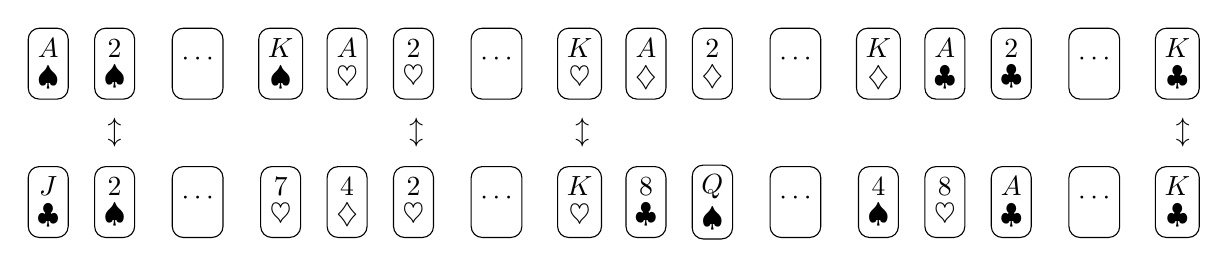
\begin{tikzpicture}
\foreach \x/\v/\s in {
  0/A/\spadesuit,
  1/2/\spadesuit,
  2.25/\cdots/,
  3.5/K/\spadesuit,
  4.5/A/\heartsuit,
  5.5/2/\heartsuit,
  6.75/\cdots/,
  8/K/\heartsuit,
  9/A/\diamondsuit,
  10/2/\diamondsuit,
  11.25/\cdots/,
  12.5/K/\diamondsuit,
  13.5/A/\clubsuit,
  14.5/2/\clubsuit,
  15.75/\cdots/,
  17/K/\clubsuit}
  \node[minimum height=9mm,draw,rounded corners]
    at (\x*24pt,0) {\shortstack{$\v$\\$\s$}};

\foreach \x/\v/\s in {
  0/J/\clubsuit,
  1/2/\spadesuit,
  2.25/\cdots/,
  3.5/7/\heartsuit,
  4.5/4/\diamondsuit,
  5.5/2/\heartsuit,
  6.75/\cdots/,
  8/K/\heartsuit,
  9/8/\clubsuit,
  10/Q/\spadesuit,
  11.25/\cdots/,
  12.5/4/\spadesuit,
  13.5/8/\heartsuit,
  14.5/A/\clubsuit,
  15.75/\cdots/,
  17/K/\clubsuit}
  \node[minimum height=9mm,draw,rounded corners]
    at (\x*24pt,-50pt) {\shortstack{$\v$\\$\s$}};

\node at (24pt,-25pt) {$\updownarrow$};
\node at (133pt,-25pt) {$\updownarrow$};
\node at (193pt,-25pt) {$\updownarrow$};
\node at (410pt,-25pt) {$\updownarrow$};
\end{tikzpicture}
\end{center}
\caption{Matching two decks of cards}\label{f.cards}
\end{figure}

\solution{}

The distribution is uniform so each card in the second row has the same probability of being matched with the card above it:
\[
E(\textsf{number of matches}) = 52\cdot \frac{1}{52} = 1\,.
\]

\newpage

\sml{}

\begin{verbatim}
Expectation of matches = 1.00
Average of matches     = 1.01
\end{verbatim}

%%%%%%%%%%%%%%%%%%%%%%%%%%%%%%%%%%%%%%%%%%%%%%%%%%%%%%%%%%%%%%%%

\begin{prob}{Probabilities of matches}

Lay out a deck of $n$ cards in order and then lay out a second deck in random order below the first row (Figure~\ref{f.cards}). Develop a formula for $P(n,r)$, the probability that there will be exactly $r$ matches of a card in the first row with the card below.

Assume that $P(k,0)$ is given for $0\leq k\leq n$.
\end{prob}

\solution{}

At first glance this problem seems to be related to Problem~28 (Catching the greedy counterfeiter) but there is a major difference. The drawings from the boxes are independent, whereas here the matches are not independent. For example, if the first match occurs on the first card (with probability $1/n$), the probability that the second card matches is $1/(n-1)$.

The probability that any \emph{given} set of $r$ cards match is:
\begin{equation}\label{eq.r-match}
\disfrac{1}{n}\cdot \disfrac{1}{n-1}\cdot \cdots \cdot \disfrac{1}{n+r-1}\,.
\end{equation}
To obtain exactly $r$ matches, Equation~\ref{eq.r-match} must be multiplied by $P(n-r,0)$, the probability that there are no matches in the remaining $n-r$ cards. Finally, there are ${n\choose r}$ ways of choosing the $r$ matches. Therefore:
\begin{eqn}
P(n,r)&=& \dischoose{n}{r}\disfrac{1}{n(n-1)(n+r-1)} P(n-r,0)\\
&=& \disfrac{n!}{r!(n-r)!}\cdot\disfrac{1}{n!/(n-r)!}P(n-r,0)\\
&=&\disfrac{1}{r!}P(n-r,0)\,,
\end{eqn}%
which solves the problem since $P(k,0)$ is given.

Mosteller develops a closed formula and a limit for $P(n,r)$:
\begin{eqnlabels}
\nonumber{}P(n,k)&=&\disfrac{1}{k!}\sum_{i=0}^{n-k} \disfrac{(-1)^i}{i!}\\
\label{eq.r-matches-lim2}
\lim_{n-r\rightarrow \infty} P(n,k)&\approx& \disfrac{1}{k!}e^{-1}\,.
\end{eqnlabels}
\sml{}

The simulation was run for $n=52$ cards and the probability computed from Equation~\ref{eq.r-matches-lim2}.
\begin{verbatim}
Probability of 1 matches = 0.3679
Proportion 1 matches     = 0.3710
Probability of 2 matches = 0.1839
Proportion 2 matches     = 0.1828
Probability of 3 matches = 0.0613
Proportion 3 matches     = 0.0569
Probability of 4 matches = 0.0153
Proportion 4 matches     = 0.0168
\end{verbatim}

%%%%%%%%%%%%%%%%%%%%%%%%%%%%%%%%%%%%%%%%%%%%%%%%%%%%%%%%%%%%%%%%

\begin{prob}{Choosing the largest dowry\annotate{D}}
Place $n$ cards face down in a row. There is a positive integer written on the face of each card but you have no knowledge of their distribution. Turn the cards over one-by-one and look at the numbers. After turning over each card you can declare that it is the largest number. If you are correct you win the game otherwise you lose.

For example, if the sequence of cards is $(47, 23, 55, 4)$ you win if and only if you choose the third card.

Make your decision according to this strategy: for some fixed $r$ reject the first $r-1$ cards and select the first card whose number is greater than all the $r-1$ cards.

\que{1} For $n=4$, $r=3$ check all permutations and determine the number of permutations where you win.

\que{2} Develop a formula for the probability of a win for arbitrary $n, r$.

\que{3} Find an approximation for the probability when $n,r\rightarrow \infty$.

\textbf{Hint:} Given $r$, in what positions can the largest number $m$ be and in what positions can the numbers less or equal to $m$ be? 

\end{prob}

\solution{}

\ans{1} 
To simplify notation we will use the rank of the numbers from low to high $1,2,\ldots,n$ although the actual numbers are not known.

There are $24$ permutations of the four numbers. By the strategy you reject the first two cards and select either the third card or the fourth card, so you lose if the  permutation has $4$ in the first two positions. What about the permutation $(1,2,3,4)$? You reject $1,2$ and select $3$ since it  greater than $1,2$, but this is not the largest card so you lose. What about the permutation $(1,3,2,4)$? Again, $1,3$ are rejected by the strategy, but $2$ is also rejected because it is \emph{not} larger than $1,3$. Now you select $4$ and win. Carry out this reasoning for all the permutations and check that permutations with boxed $4$s are wins (Table~\ref{t.dowry}). The probability of winning is $10/24$.
\begin{table}[tb]
\[
\addtolength{\arraycolsep}{-2pt}
\renewcommand*{\arraystretch}{1.5}
\begin{array}{cc|cc@{\hspace{2em}}cc|cc@{\hspace{2em}}cc|cc@{\hspace{2em}}cc|cc@{\hspace{2em}}cc|cc@{\hspace{2em}}cc|cc}
1&2\;&\;3&4&
1&2\;&\;\fbox{4}&3&
1&3\;&\;2&\fbox{4}&
1&3\;&\;\fbox{4}&2&
1&4\;&\;2&3&
1&4\;&\;3&2\\
2&1\;&\;3&4&
2&1\;&\;\fbox{4}&3&
2&3\;&\;1&\fbox{4}&
2&3\;&\;\fbox{4}&1&
2&4\;&\;1&3&
2&4\;&\;3&1\\
3&1\;&\;2&\fbox{4}&
3&1\;&\;\fbox{4}&2&
3&2\;&\;1&\fbox{4}&
3&2\;&\;\fbox{4}&1&
3&4\;&\;1&2&
3&4\;&\;2&1\\
4&1\;&\;2&3&
4&1\;&\;3&2&
4&2\;&\;1&3&
4&2\;&\;3&1&
4&3\;&\;1&2&
4&3\;&\;2&1
\end{array}
\]
\caption{Largest dowry for $n=4,r=3$}\label{t.dowry}
\end{table}


\ans{2} If the largest number is in one of the positions $1,\ldots,r-1$ you lose. Therefore, in order to win the largest number must be in the $m$th position for $r\leq m\leq n$:
\[
1\quad 2\quad \cdots\quad r-2 \quad r-1 \quad \overbrace{r \quad r+1 \quad \cdots\quad m-1\quad  m \quad m+1\quad \cdots \quad n}^{\textsf{largest must be here}}
\]
By the strategy you reject the first $r-1$ cards. You will choose position $m$ only if \emph{all} the numbers in $(r,\ldots,m-1)$ are less than or equal to \emph{all} the numbers in $(1,\ldots,r)$. In other words, the largest card in the sequence $(1,\ldots,m-1)$ is \emph{not} in the second part of the sequence $(r,\ldots m-1)$ but in the first part $(1,\ldots,r-1)$. The probability is:
\[
P(\textsf{largest number in}\;(1,\ldots,m-1)\;\textsf{is in}\; (1,\ldots,r-1)) = \disfrac{r-1}{m-1}\,.
\]

This reasoning will be easier to follow in an example. Given the numbers $1,\ldots,10$ and $r=5$:
\[
2\quad \quad 5\quad \quad 6\quad \quad 3 \quad \quad  \overbrace{1 \quad \quad 4 \quad \quad 9 \quad \quad 10\quad\quad 8}^{\textsf{largest must be here}}
\]
The largest number is at position $m=9$. However the largest number in $(1,\ldots,m-1=8)$ is \emph{in} the sequence $(r=5,\ldots,m-1=8)$ so you will not win. By the strategy you will select $9$, the first number larger that all those in $(1,\ldots,r-1=4)$ and lose because $10>9$. If, however, the places of $9$ and $10$ were exchanged, then the largest number less than $10$ is $6$ at position $3<r=5$, so by the strategy you will not select $1,4$ and you will win:
\[
\begin{array}{l}
\overbrace{2\quad \quad 5\quad \quad 6\quad \quad 3}^{\textsf{here}} \quad \quad  \overbrace{1 \quad \quad 4 \quad \quad \mathbf{9}}^{\textsf{not here}}  \quad \quad 10\quad\quad 8\\
\overbrace{2\quad \quad 5\quad \quad \mathbf{6}\quad \quad 3}^{\textsf{here}} \quad \quad  \overbrace{1 \quad \quad 4}^{\textsf{not here}} \quad \quad 10  \quad \quad 9\quad\quad 8
\end{array}
\]

Since the probability that the largest number is at $m$ is $1/n$:
\begin{equation}\label{eq.dowry1}
P(\textsf{win}) = \sum_{m=r}^{n} \disfrac{1}{n} \cdot \disfrac{r-1}{m-1}= \disfrac{r-1}{n}\sum_{m=r}^{n} \disfrac{1}{m-1}\,.
\end{equation}
For $n=4, r=3$, $P(\textsf{win}) =5/12=10/24$, the result found by checking all permutations.

\ans{3}
Rewrite Equation~\ref{eq.dowry1} as:
\begin{equation}\label{eq.dowry2}
P(\textsf{win}) =\disfrac{r-1}{n}\left(\sum_{m=2}^{n} \disfrac{1}{m-1}-\sum_{m=2}^{r-1} \disfrac{1}{m-1}\right)\,.
\end{equation}
For large $n,r$, the two harmonic series Equation~\ref{eq.dowry2} can be approximated by:
\begin{equation}\label{eq.dowry3}
P(\textsf{win})=\disfrac{r}{n}(\ln n - \ln r)=\disfrac{r}{n}\ln \disfrac{n}{r}=-\disfrac{r}{n}\ln \disfrac{r}{n}\,.
\end{equation}
Denote $x=r/n$ and find the maximum by taking derivatives:
\begin{eqn}
(-x\ln x)' &=& -x\cdot \frac{1}{x} + (-1) \ln x=0\\
\ln x &=& -1\\
x &=& 1/e\,.
\end{eqn}%
Therefore, to maximize that probability of winning choose $r \approx n/e$ and from Equation~\ref{eq.dowry3}:
\[
P(\textsf{win})\approx-\disfrac{1}{e}\ln\left(\disfrac{1}{e}\right)=\disfrac{1}{e}\approx \disfrac{1}{3}\,,
\]
much larger than the probability $1/n$ of winning by picking a random card.

\sml{}
The simulation was run with $100$ cards and values of $r$ near $100/e$:
\begin{verbatim}
Reject cards before r = 36:
Probability of wins   = 0.3674
Proportion wins       = 0.3678
Reject cards before r = 37:
Probability of wins   = 0.3678
Proportion wins       = 0.3767
Reject cards before r = 38:
Probability of wins   = 0.3679
Proportion wins       = 0.3638
Reject cards before r = 39:
Probability of wins   = 0.3677
Proportion wins       = 0.3763
\end{verbatim}

%%%%%%%%%%%%%%%%%%%%%%%%%%%%%%%%%%%%%%%%%%%%%%%%%%%%%%%%%%%%%%%%

\begin{prob}{Choosing the largest random number\annotate{D}}

Place $n$ cards face down in a row. There is a real number  written on the face of each card with a uniform distribution in $[0.0,1.0]$. Turn the cards over one-by-one and look at the numbers. After turning over each card you can declare that it is the largest number. If you are correct you win the game otherwise you lose. 

Use the strategy of Problem~47: for some fixed $r$ reject the first $r-1$ cards and select the first card whose number is greater than all the $r-1$ cards.

\textbf{Definition:} $d$, the \emph{indifference value}, is the value of a card below which you decide to reject that card and above which you decide to select it.

\que{1} For $n=1$ compute the indifference value for the first card and compute the probability of winning.

\que{2} For $n=2$ compute the indifference value for the first card and compute the probability of winning.

\que{3} For $n=3$ compute the indifference value for the first card and compute the probability of winning. Do not try to compute the probability of winning!

\textbf{Note:} In Problem~37 the values could be $100, 200, 300$ or $100, 50, 20$, so uncovering the first number gives no information about the other numbers. In this problem since the distribution is uniform if the first number is $0.3$ the probability that the second number is smaller is $0.3$ and the probability that it is larger is $0.7$.
\end{prob}

\solution{}

Let $v_1,v_2,v_3$ be the values of the three cards.

\ans{1} You have no choice but to select the first card since there are no other cards. There is no indifference value. $v_1$ is the ``largest'' number and $P({win})=1$.

\ans{2} If you select the first card, $P(\textsf{win})=v_1$ because $v_1$ is the probability that the second card has a smaller value. If you reject the first card, $P(\textsf{win})=1-v_1$ because $1-v_1$ is the probability that $v_2>v_1$. Therefore, if $v_1<0.5$ select the second card because $1-v_1>0.5$ and if $v_1>0.5$ select the first card because $1-v_1<0.5$. By definition, the indifference value is $d=0.5$ since we have shown that the decision to select changes depending on whether $v_1$, the value of card, is above or below $d$.

The probability of winning is:
\begin{equation}\label{eq.largest-random1}
P(\textsf{win}) = P(\textsf{win} \,|\,v_1<0.5)\,P(v_1<0.5)+ P(\textsf{win}\,|\,v_1>0.5)\,P(v_1>0.5)\,.
\end{equation}
$P(v_1<0.5)=0.5$ follows by the uniform distribution. What about $P(\textsf{win} \,|\,v_1<0.5)$? By the strategy you win if $0.5<v_2<1$, but you also win if $v_1<v_2<0.5$. Since $v_1$ is uniformly distributed in $(0,0.5)$ the probability that $v_1<v_2<0.5$ is one-half the range:
\[
P(\textsf{win} \,|\,v_1<0.5)=0.50+0.25=0.75\,.
\]
A similar computation holds for $v_1>0.5$ and from Equation~\ref{eq.largest-random1} we have:
\[
P(\textsf{win})=0.75\cdot 0.50 + 0.75\cdot 0.50=0.75\,.
\]

\ans{3}

If you select the first card, $P(\textsf{win})=v_1^2$ because the second and third cards must be smaller than the first.

If you reject the first card and select the next card larger than $v_1$ then:
\begin{itemize}
\item $P(\textsf{win})=v_1(1-v_1)$ if $v_2<v_1$ (reject $v_2$) and $v_3>v_1$ (select $v_3$ and win).
\item $P(\textsf{win})=(1-v_1)v_1$ if $v_2>v_1$ (select $v_2$) and $v_3<v_1$ (win since $v_3<v_2$).
\item $P(\textsf{win})=\frac{1}{2}(1-v_1)^2$ if $v_2>v_1$ (select $v_2$) and $v_3>v_1$. The factor of $1/2$ takes into account that winning depends on whether $v_3<v_2$ (win) or $v_2<v_3$ (lose).
\end{itemize}

The indifference value $d$ of the first card is the value of the card such that the probability of winning by selecting it equals the probability of winning by rejecting it:
\begin{eqn}
d^2 &=& d(1-d)+(1-d)d + \frac{1}{2}(1-d)^2\\
5d^2 - 2d -1 &=&0\\
d&=& \disfrac{1+\sqrt{6}}{5}\approx 0.6899\,.
\end{eqn}%
Gilbert and Mosteller \cite[page~55]{gilbert} show that for $n=3$:
\[
P(\textsf{win}) = \disfrac{1}{3}+\disfrac{d}{2}+\disfrac{d^2}{1}-\disfrac{3d^3}{2}\approx 0.6617\,.
\]
\textbf{Simulation:}
\begin{verbatim}
For  3 cards:
Indifference value = 0.6000
Probability of win = 0.6693
Proportion of wins = 0.6628
Indifference value = 0.6899
Probability of win = 0.6617
Proportion of wins = 0.6711
Indifference value = 0.7200
Probability of win = 0.6519
Proportion of wins = 0.6473
\end{verbatim}

%%%%%%%%%%%%%%%%%%%%%%%%%%%%%%%%%%%%%%%%%%%%%%%%%%%%%%%%%%%%%%%%

\begin{prob}{Doubling your accuracy}
You are given two rods of lengths $L_1>L_2$ and a length-measuring instrument whose possible error is given by a normal distribution\footnote{This problem assumes that the reader is familiar with normal distributions.} with mean $0$ and variance $\sigma^2$. The lengths of the two rods can be measured by measuring each one separately. Is there a more accurate method?
\end{prob}

\newpage

\solution{}

\begin{figure}[bt]
\begin{center}
\begin{tikzpicture}
\draw (0,0) -- ++(8,0) -- ++(0,12pt) -- ++(-8,0) -- cycle;
\draw[<->] (0,24pt) --
  node[fill=white] {$\scriptstyle L_1+L_2$} ++(14,0);
\draw (8,0) -- ++(6,0) -- ++(0,12pt) -- ++(-6,0) -- cycle;
\begin{scope}[yshift=-48pt]
\draw[yshift=12pt] (0,0) -- ++(8,0) -- ++(0,12pt) -- ++(-8,0) -- cycle;
\draw (0,0) -- ++(0,12pt) -- ++(6,0) -- ++(0,-12pt) -- cycle;
\draw[<->] (6,4pt) --
  node[fill=white] {$\scriptstyle L_1-L_2$} ++(2,0);
\end{scope}
\end{tikzpicture}
\end{center}
\caption{Measuring the lengths of two rods}\label{f.rods}
\end{figure}
Place the rods end-to-end and measure $L_s=L_1+L_2$ and then place the rods side-by-side and measure $L_d=L_2-L_1$ (Figure~\ref{f.rods}). Compute $L_1,L_2$:
\begin{eqn}
\textstyle\frac{1}{2}(L_s+L_d)&=&\textstyle\frac{1}{2}((L_1+L_2)+(L_1-L_2))=L_1\\
\textstyle\frac{1}{2}(L_s-L_d)&=&\textstyle\frac{1}{2}((L_1+L_2)-(L_1-L_2))=L_2\,.
\end{eqn}%%
Let $e_s$ be the mean error of $L_s$ and $e_d$ the mean error of $L_d$. Then:
\begin{eqn}
\textstyle\frac{1}{2}((L_s+e_s)+(L_d+e_d))&=&L_1+\textstyle\frac{1}{2}(e_s+e_d)\\
\textstyle\frac{1}{2}((L_s+e_s)-(L_d+e_d))&=&L_2+\textstyle\frac{1}{2}(e_s-e_d)\,.
\end{eqn}%
Since the means of $e_s, e_d$ are $0$, the means of $\frac{1}{2}(e_s+e_d)$ and $\frac{1}{2}(e_s-e_d)$ are also $0$, so this method of measurement is no more accurate. However, the variance is of the measurements are reduced to half their previous values:\footnote{The measurements are independent so the covariance is $0$.}
\begin{eqn}
\mathrm{Var}\left(\textstyle\frac{1}{2}\left(L_s+L_d\right)\right)&=&
  \textstyle\frac{1}{4}(\sigma^2+\sigma^2)=\frac{1}{2}\sigma^2\\
\mathrm{Var}\left(\textstyle\frac{1}{2}(L_s-L_d)\right)&=&
  \textstyle\frac{1}{4}( \sigma^2+(-1)^2\sigma^2)=\frac{1}{2}\sigma^2\,.
\end{eqn}%

\sml{}

\begin{verbatim}
For L1 = 40, L2 = 16, variance = 0.50:
L1 mean = 39.9907, L1 variance = 0.2454
L2 mean = 16.0030, L2 variance = 0.2520

For L1 = 40, L2 = 16, variance = 1.00:
L1 mean = 39.9934, L1 variance = 0.4949
L2 mean = 15.9889, L2 variance = 0.4878

For L1 = 40, L2 = 16, variance = 2.00:
L1 mean = 39.9924, L1 variance = 0.9940
L2 mean = 16.0104, L2 variance = 1.0069
\end{verbatim}
The means are very accurate and the variances are halved for $\sigma^2=0.5,\sigma^2=1.0$ but the variance is not affected for $\sigma^2=2.0$.

%%%%%%%%%%%%%%%%%%%%%%%%%%%%%%%%%%%%%%%%%%%%%%%%%%%%%%%%%%%%%%%%

\begin{prob}{Random quadratic equations}

Consider the quadratic equation $x^2+2bx+c=0$ defined on $[-B,B]\times[-B,B]$ for $B\geq 1$.

\que{1} What is the probability that the roots are real?

\que{2} As $B\rightarrow \infty$ what is the probability that the roots are real?
\end{prob}

\solution{}

\ans{1}
The roots will be real if the discriminant is non-negative: $4b^2-4c\geq 0$. Figure~\ref{f.real-roots} shows a plot of the parabola $c=b^2$ where the complex roots are within the shaded area. For example, for $(b,c)=(1,2)$, denoted by the red dot, $x^2+2x+2$ has complex roots $-1\pm i\sqrt{3}$, while for $(b,c)=(2,2)$, denoted by the blue dot, $x^2+4x+2$ has real roots $-2\pm \sqrt{2}$.
\begin{figure}[tb]
\begin{center}
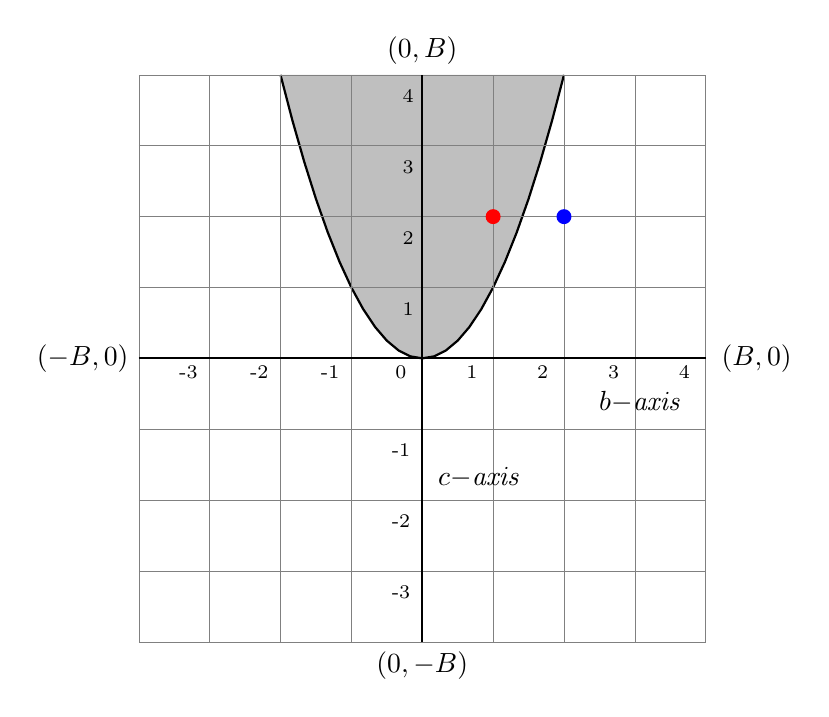
\begin{tikzpicture}[scale=.9]
\fill [white!50!gray, domain=-2:2]
      (-2, 4) -- plot ({\x}, {\x*\x}) -- (2, 4) -- cycle;
\draw [thick, domain=-2:2]
      (-2, 4) -- plot ({\x}, {\x*\x}) -- (2, 4);
\draw[help lines] (-4,-4) grid (4,4);
\draw[thick] (-4,0) -- (4,0);
\draw[thick] (0,-4) -- (0,4);
\foreach \x in {-3,...,4}
  \node at (\x-.3,-.2) {\scriptsize \x};
\foreach \y in {1,...,4}
  \node at (-.2,\y-.3) {\scriptsize \y};
\foreach \y in {-3,...,-1}
  \node at (-.3,\y-.3) {\scriptsize \y};
\draw[thick] (0,-4) node[below] {$(0,-B)$} -- 
  node[right,near start,xshift=2pt,yshift=8pt]
  {$c\mathit{-axis}$} (0,4) node[above] {$(0,B)$};
\draw[thick] (-4,0) node[left] {$(-B,0)$} --
  node[below,very near end,xshift=2pt,yshift=-8pt] 
  {$b\mathit{-axis}$} (4,0) node[right,xshift=2pt] {$(B,0)$};
\fill[red] (1,2) circle(3pt);
\fill[blue] (2,2) circle(3pt);
\end{tikzpicture}
\end{center}
\caption{For $(b,c)$ in the shaded area the roots of $x^2+2bx+c$ are complex}\label{f.real-roots}
\end{figure}

The shaded area can be computed by integration:
\[
\int_{-\sqrt{B}}^{\sqrt{B}} (B-b^2)\,db=
\left. Bb-\disfrac{b^3}{3}\right|_{-\sqrt{B}}^{\sqrt{B}}=
\left(B^{3/2}-\frac{B^{3/2}}{3}\right)-
\left(-B^{3/2}+\frac{B^{3/2}}{3}\right)=
\disfrac{4}{3}B^{3/2}\,.
\]
The total area of the range $[-B,B]\times[-B,B]$ is $4B^2$ so:
\begin{eqn}
P(\textsf{complex roots})&=&\disfrac{\frac{4}{3}B^{3/2}}{4B^2}=\disfrac{1}{3\sqrt{B}}\\
P(\textsf{real roots})&=&1-\disfrac{1}{3\sqrt{B}}\,.
\end{eqn}%
\ans{2}
\[
\lim_{B\rightarrow\infty}
P(\textsf{real roots})=
\lim_{B\rightarrow\infty} \left(1-\disfrac{1}{3\sqrt{B}}\right)=
1\,.
\]

\sml{}
\begin{verbatim}
For B =  4:
Probability of real roots = 0.8333
Proportion real roots     = 0.8271
For B = 16:
Probability of real roots = 0.9167
Proportion real roots     = 0.9205
For B = 64:
Probability of real roots = 0.9583
Proportion real roots     = 0.9582
\end{verbatim}

%%%%%%%%%%%%%%%%%%%%%%%%%%%%%%%%%%%%%%%%%%%%%%%%%%%%%%%%%%%%%%%%

\begin{prob}{Two-dimensional random walk\annotate{D}}
A particle is placed at the origin of a two-dimensional coordinate system. The particle moves left or right on the $x$-axis with probabilities $1/2$ for each direction and \emph{simultaneouly} up or down the $y$-axis with probabilities $1/2$ for each direction. Figure~\ref{f.2d-random-walk} shows a random walk of $22$ steps starting at and returning to the origin.

\que{1} What is the probability that the particle returns to the origin in two moves?

\que{2} Develop a formula for the expectation of the number of visits of the particle to the origin.

\que{3} Use Stirling's approximation to estimate the number of visits of the particle to the origin for large $n$.

\textbf{Hint} Use indicator variables to compute the expectation.

\begin{figure}[t]
\begin{center}
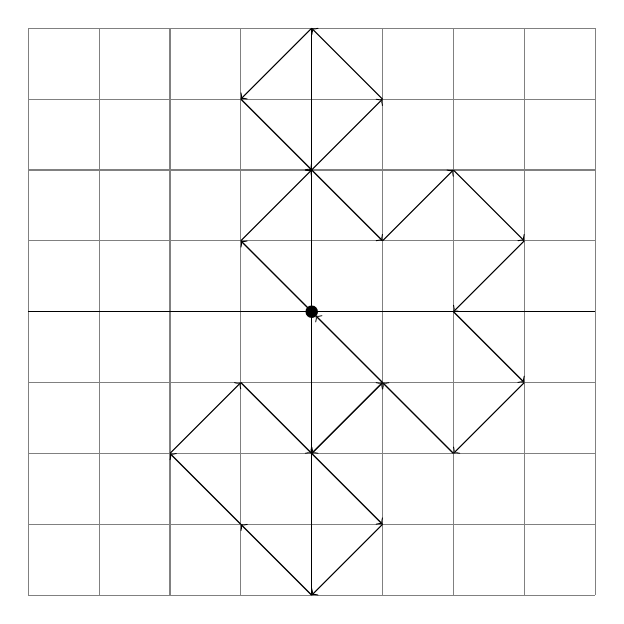
\begin{tikzpicture}[scale=.9]
\draw[color=gray] (-4,-4) grid (4,4);
\draw (-4,0) -- (4,0);
\draw (0,-4) -- (0,4);
\fill (0,0) circle[radius=2.5pt];
\draw[->] (0,0)  -- (-1,1);
\draw[->] (-1,1) -- (0,2);
\draw[->] (0,2)  -- (1,3);
\draw[->] (1,3)  -- (0,4);
\draw[->] (0,4)  -- (-1,3);
\draw[->] (-1,3) -- (0,2);
\draw[->] (0,2)  -- (1,1);
\draw[->] (1,1)  -- (2,2);
\draw[->] (2,2)  -- (3,1);
\draw[->] (3,1)  -- (2,0);
\draw[->] (2,0)  -- (3,-1);
\draw[->] (3,-1) -- (2,-2);
\draw[->] (2,-2) -- (1,-1);
\draw[->] (1,-1) -- (0,-2);
\draw[->] (0,-2) -- (1,-3);
\draw[->] (1,-3) -- (0,-4);
\draw[->] (0,-4) -- (-1,-3);
\draw[->] (-1,-3)-- (-2,-2);
\draw[->] (-2,-2)-- (-1,-1);
\draw[->] (-1,-1)-- (0,-2);
\draw[->] (0,-2) -- (1,-1);
\draw[->] (1,-1) -- (.055,-.055);
\end{tikzpicture}
\end{center}
\caption{Two-dimensional random walk}\label{f.2d-random-walk}
\end{figure}
\end{prob}

\solution{}

\ans{1}
The dots in Figure~\ref{f.two-moves} show the possible positions of the particle after two moves:
\begin{itemize}
\item The green path shows a move to $(\pm 2, \pm 2)$ by taking two moves in the same direction. The probability is $\left(\frac{1}{4}\right)^2= \frac{1}{16}$.
\item The red path shows a move to $(\pm 2,0)$ or $(0,\pm 2$). There are two possible paths for each one so the probability is $2\cdot\left(\frac{1}{4}\right)^2= \frac{2}{16}$.
\item The blue path shows a move to $(\pm 1,\pm 1)$ and back to the origin. The probability is $\frac{1}{16}$.
\end{itemize}
Let $P_{2n}(x,y)$ be the probability that the particle reaches $(x,y)$ in $2n$ moves.

The four possible blue paths are the only ones that return to the origin so:
\[
P_{2}(0,0)=\frac{4}{16}\,.
\]

\begin{figure}[tb]
\begin{center}
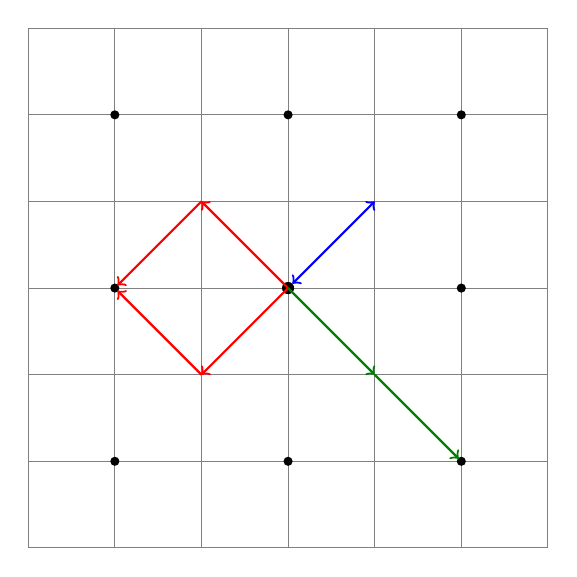
\begin{tikzpicture}[scale=1.1]
\draw[color=gray] (-3,-3) grid (3,3);
\fill (0,0) circle[radius=2pt];
\foreach \x/\y in {2/2, 2/-2, -2/2, -2/-2, 
                   0/2, 0/-2, 2/0, -2/0}
  \fill (\x,\y) circle[radius=1.5pt];
\draw[->,red,thick] (0,0) -- (-1,-1);
\draw[->,red,thick] (-1,-1) -- (-1.97,-.03);
\draw[<-,red,thick] (-1.97,0.03) -- (-1,1);
\draw[<-,red,thick] (-1,1) -- (0,0);
\draw[->,green!50!black,thick] (0,0) -- (1,-1);
\draw[->,green!50!black,thick] (1,-1) -- (1.97,-1.97);
\draw[<->,blue,thick] (.05,.05) -- +(.95,.95);
\end{tikzpicture}
\end{center}
\caption{Two moves of the random walk}\label{f.two-moves}
\end{figure}

\ans{2} The choice of direction for both axes are independent:
\begin{equation}\label{eq.2d-1}
P_{2n}(0,0) =
P_{2n}(0,b)\cdot P_{2n}(a,0)\,,
\end{equation}
where $a,b$ are arbitrary integers.

The particle will return to the origin if and only if for both axes the number of $+1$ moves equals the number of $-1$ moves. There are ${2n \choose n}$ ways to arrange $n$ moves of $+1$ and $n$ moves of $-1$ so:
\begin{eqnlabels}
\nonumber{}P_{2n}(0,b) =P_{2n}(a,0)&=&
\dischoose{2n}{n}\left(\disfrac{1}{2}\right)^n\left(\disfrac{1}{2}\right)^{n}\\
\label{eq.return-to-origin1}P_{2n}(0,0) &=&
\left[\dischoose{2n}{n}\left(\disfrac{1}{2}\right)^{2n}\right]^2\,.
\end{eqnlabels}%
Define the indicator variables $I_{2n}(0,0)$ for returning to the origin in $2n$ steps and let $E(0,0)$ the expectation of the \emph{number of returns to the origin} in any number of steps. Now:
\[
E(0,0) = \sum_{n=1}^{\infty}E(I_{2n}(0,0))\,.
\]
You might ask what happens if the particle takes three steps and then returns to the origin and again takes three steps and returns to the origin. Shouldn't $I_6(0,0)$ have the value two and not one? The answer is that on the second return the particle has taken $12$ steps which will be counted by $I_{12}(0,0)=1$.

From Equations~\ref{eq.expectation-prob},~\ref{eq.expectation-sum}:
\begin{equation}
E(0,0) =
\sum_{n=1}^{\infty}E(I_{2n}(0,0)) =
E\left(\sum_{n=1}^{\infty}I_{2n}(0,0)\right) =
\sum_{n=1}^{\infty}P_{2n}(0,0) =
\sum_{n=1}^{\infty}\left[\dischoose{2n}{n}\left(\disfrac{1}{2}\right)^{2n}\right]^2\,.\label{eq.return-to-origin2}
\end{equation}

\ans{3}
By Stirling's approximation $n! \approx \sqrt{2\pi n}\left(n/e\right)^n$:
\begin{eqnlabels}
\nonumber E_{2n}(0,0) &=&
\left[\dischoose{2n}{n}
\left(\disfrac{1}{2}\right)^{2n}\right]^2 \\
\nonumber{}&=&
\left[\disfrac{(2n)!}{n!n!}
\left(\disfrac{1}{2}\right)^{2n}\right]^2 \\
\nonumber{}&\approx&
\left(\disfrac{1}{2}\right)^{4n}
\disfrac{(\sqrt{2\pi \cdot 2n})^2
         \left(2n/e\right)^{4n}}
        {(\sqrt{2\pi n})^{4}
         \left(n/e\right)^{4n}} \\
\nonumber{}&=&\left(\disfrac{1}{2}\right)^{4n}\disfrac{4\pi n}{4\pi^2 n^2}\cdot
\disfrac{\left(n/e\right)^{4n}\cdot 2^{4n}}{\left(n/e\right)^{4n}}\\
\nonumber{}&=& \disfrac{1}{\pi n}\\
\label{eq.rw-2d}E(0,0) &=& \disfrac{1}{\pi}\sum_{n=1}^{\infty}\disfrac{1}{n}\,,
\end{eqnlabels}%
which is the the harmonic series that diverges so with probability $1$ the particle returns to the origin!

Since $E(0,0)=\infty$ the number of times that the particle returns to origin is unbounded. However, by the first axiom of probability (page~\pageref{p.first-axiom}), $P(0,0)$, the probability that the particle will return to the origin, must satisfy $0\leq P(0,0) \leq 1$ so $P(0,0)=1$, meaning that it is certain that the particle returns to the origin. In general, the expectation of a random variable is infinite if and only if its probability is one.

\sml{}

The simulation was run one hundred times for one million steps each.
\begin{verbatim}
Proportion returned to origin = 0.8700
\end{verbatim}
Since the probability of returning to the origin is $1$ the result should be close to $1.0000$. The result obtained can be interpreted to mean that although every particle will return to the origin, it can take an extremely large number of steps to do so.

%%%%%%%%%%%%%%%%%%%%%%%%%%%%%%%%%%%%%%%%%%%%%%%%%%%%%%%%%%%%%%%%

\begin{prob}{Three-dimensional random walk\annotate{D}}
A particle is placed at the origin of a three-dimensional coordinate system. The particle moves left or right on the $x$-axis with probabilities $1/2$ \emph{and} up or down the $y$-axis with probabilities $1/2$ \emph{and} in or out on the $z$-axis with probabilities $1/2$.

\que{1} Develop a formula for the expectation of the number of times that the particle returns to the origin and estimate its value using Stirling's approximation.

\textbf{Hint:} Develop a formula for the probability and then use indicator variables.

\que{2} What is the probability that the particle will return to the origin \emph{at least once}?

\textbf{Hint:} Use the technique from Problem~4.
\end{prob}

\solution{}

\ans{1} $P_{2n}(0,0,0)$, probability of returning to the origin after $2n$ steps, is given by generalizing Equation~\ref{eq.return-to-origin1} to three dimensions:
\begin{equation}\label{eq.rw-multiply}
P_{2n}(0,0,0) =
P_{2n}(0,a,b)\cdot P_{2n}(c,0,d)\cdot P_{2n}(e,f,0)\,.
\end{equation}
$E(0,0)$, the expectation of the number of returns of the particle to the origin, is given by the analogue of Equation~\ref{eq.return-to-origin2}:
\begin{eqnarray*}
E(0,0,0) &=&
\sum_{n=1}^{\infty}E(I_{2n}(0,0,0))\\
& =&E\left(\sum_{n=1}^{\infty}I_{2n}(0,0,0)\right) \\
&=&\sum_{n=1}^{\infty}P_{2n}(0,0,0)\\
& =&\sum_{n=1}^{\infty}\left[\dischoose{2n}{n}\left(\disfrac{1}{2}\right)^{2n}\right]^3\,.
\end{eqnarray*}

From Stirling's approximation:
\begin{eqnlabels}
\nonumber{}P_{2n}(0,0,0) &=&
\left[\disfrac{(2n)!}{(n!)^2}
\left(\disfrac{1}{2}\right)^{2n}\right]^3 \\
\nonumber{}&\approx&
\left(\disfrac{1}{2}\right)^{6n}
\disfrac{(\sqrt{2\pi \cdot 2n})^3
         \left(2n/e\right)^{6n}}
        {(\sqrt{2\pi n})^{6}
         \left(n/e\right)^{6n}} \\
\nonumber{}&=& \disfrac{1}{(\pi n)^{3/2}}\\
\label{eq.rw-3d}E(0,0,0) &=& \sum_{n=1}^{\infty}\disfrac{1}{(\pi n)^{3/2}}\approx 0.3772\,.
\end{eqnlabels}%
Mosteller used $18$ terms in his computation of the sum of the series and obtained $0.315$. My program used $500$ terms and obtained $0.3772$.

\que{2} Let $P_1$ be the probability that the particle returns to the origin \emph{at least once}.  From Problem~4 we know that the expectation of the number of trials until the first one where the particle \emph{does not} return to the origin is $1/(1-P_1)$. Therefore, the expectation of the number of trials for which the particle does return to the origin is one less, because the particle can return to the origin many times until finally it does not \cite{montgomery}. It follow that:
\begin{eqn}
E(0,0,0) &=& \disfrac{1}{1-P_1} - 1\\
P_1&=& \disfrac{E(0,0,0)}{1+E(0,0,0)}\,.
\end{eqn}%
In \ansnc{1} we computed that $E(0,0,0)\approx 0.3772$ so:
\[
P_1 \approx 1- \disfrac{1}{1+0.3772}
\approx 0.2739\,.
\]
\sml{}
\begin{verbatim}
Expectation of reaching origin = 0.3772
Average times reached origin   = 0.3630
Probability of reaching origin = 0.2739
Proportion reached origin      = 0.2790
\end{verbatim}

\textbf{Higher dimensions:} Equation~\ref{eq.rw-multiply} can be extended to any number of dimensions and from Equations~\ref{eq.rw-2d}, \ref{eq.rw-3d}, it is reasonable to conjecture that $E(0,0,0)$ is \emph{proportional to}:
\begin{equation}
\label{eq.rw-sum}
\sum_{n=1}^{\infty} \disfrac{1}{n^{d/2}}\,,
\end{equation}
where $d$ is the dimension \cite{louigi}. Now use the \emph{Cauchy condensation test} \cite{wiki:cauchy} on Equation~\ref{eq.rw-sum}:
\[
\sum_{n=1}^{\infty} \disfrac{1}{n^{d/2}} \quad \textsf{converges if and only if} \quad \sum_{n=1}^{\infty} \disfrac{2^n}{(2^n)^{d/2}} \quad \textsf{converges}\,.
\]
For $d=2$ the result is $\sum_{n=1}^{\infty} 1$ which clearly diverges.

For $d=3$, $E(0,0,0)$ converges since:
\[
\sum_{n=1}^{\infty} \disfrac{2^n}{(2^n)^{3/2}}=\sum_{n=1}^{\infty} \disfrac{2^n}{2^n\cdot 2^{n/2}}=\sum_{n=1}^{\infty} \disfrac{1}{(\sqrt{2})^n}=\frac{1}{\sqrt{2}-1}\approx 2.4\,.
\]
For $d=4$, $E(0,0,0,0)$ converges since $\sum_{n=1}^{\infty} \frac{1}{2^n}=2$.

For higher dimensions the expectation of the number of returns to the origin is finite but decreasing, so it becomes less and less likely that the particle will return in any particular 3D random walk.

%%%%%%%%%%%%%%%%%%%%%%%%%%%%%%%%%%%%%%%%%%%%%%%%%%%%%%%%%%%%%%%%

\begin{prob}{Buffon's needle\annotate{D}}
Consider a needle of length $a\leq 1$ and a surface ruled with parallel lines $1$ apart.\footnote{Mosteller uses $l$ as the length of the needle and $a$ as one-half the distance between the parallel lines. The problem has been simplified by specifying that the distance between the lines as $1$. We ignore the possibilities that the needle lies on a line or just touches two lines since the probability of these events is zero.} Throw the needle onto the surface. What is the probability that the needle crosses a line?

\textbf{Hint:} There are two independent random variables (Figure~\ref{f.buffon1}): $x$, the distance of the center of the needle $C$ from the closest line which is uniformly distributed in the range $[0,1/2]$, and $\theta$, the angle between the needle and the parallel lines which is uniformly distributed in the range $[0,\pi/2]$.

\begin{figure}[tb]
\begin{center}
\begin{tikzpicture}[scale=1]
\draw (0,0) -- (10,0);
\draw (0,4) -- (10,4);
\draw[<->] (1,0) -- node[fill=white] {$1$} (1,4);
\coordinate (center) at ($(4,-.5)+(60:1.8)$);
\node[above right,xshift=4pt] at (center) {$\theta$};
\fill (center) circle [radius=2pt] node[above left] {$C$};
\draw[thick] (4,-.5) -- node[left,very near end] {$a$} +(60:3.6);
\draw[thick,dashed] ($(center)+(-2,0)$) -- +(6,0);
\draw[<->] (7,0) -- node[fill=white] {$x$}
  (center -| 7,0);
\end{tikzpicture}
\end{center}
\caption{Buffon's needle}\label{f.buffon1}
\end{figure}
\end{prob}

\solution{1}

Let $p(a)$ be the probability that a needle of length $a$ crosses a line and define the indicator variable:
\[
I_{\textsf{crosses}}=
\left\{
\begin{array}{ll}
1,\quad \textsf{if a needle of length}\;a\;\textsf{crosses a line}\\
0, \quad \textsf{if a needle of length}\;a\;\textsf{does not cross a line}\,.
\end{array}
\right.
\]
Then:
\begin{equation}\label{eq.buffon-probability}
E(I_{\textsf{crosses}})=1\cdot p(a) + 0\cdot (1-p(a))=p(a)\,,
\end{equation}
and the probability can be computed by computing the expectation.

Let $m$ be a line perpendicular to the parallel lines that passes through the center of the needle $C$ and let $\theta$ be the angle between the needle and a parallel line. Project the needle onto $m$ to give the line segment $\overline{DE}$. The probability that the needle will cross a line is:
\begin{equation}\label{eq.cross}
P(\textsf{needle of length}\;a,\;\textsf{angle}\;\theta\;\textsf{crosses line})=\disfrac{\overline{CE}}{1/2}=\disfrac{(a/2)\sin \theta}{1/2}=a\sin\theta\,.
\end{equation}

\begin{figure}[b]
\begin{center}
\begin{tikzpicture}[scale=1]
\draw (0,0) -- (10,0);
\draw (0,4) -- (10,4);
\draw[<->] (1,0) -- node[fill=white,yshift=12pt] {$1$} (1,4);

\coordinate (center) at ($(4,-.5)+(60:1.8)$);
\fill (center) circle [radius=2pt] node[above left] {$C$};

\coordinate (end1) at ($(center)+(60:1.8)$);
\draw[thick] (center) -- node[right,near end,yshift=1pt]
 {$a/2$} (end1) node[above right] {$D$};
\coordinate (end2) at ($(center)+(60:-1.8)$);
\draw[thick] (center) -- node[left] {$a/2$} (end2)
  node[below left] {$E$};

\draw[thick,dashed] ($(center)+(-2,0)$) -- +(6,0);
\draw[<->] (8,0) -- node[fill=white] {$x$}
  (center -| 8,0);
\draw[thick,dotted] (0,2) -- (10,2);
\draw[<->] (2.25,0) -- node[fill=white] {$1/2$} +(0,2);

\draw[thick,dashed] ($(center)+(0,-2)$) --
  node[right,near end,xshift=-1pt,yshift=16pt]
  {$m$} +(0,4.8);

\draw[thick] (end1)-- (end1 -| center) --
  node[left,yshift=12pt] {$(a\sin\theta)/2$}
  (center);
\draw[thick] (end2) -- (end2 -| center) -- 
  node[right] {$(a\sin \theta)/2$} (center);

\node[above right,xshift=4pt] at (center) {$\scriptstyle\theta$};
\node[below left,xshift=-2pt,yshift=2pt] at (end1) 
  {$\scriptstyle\theta$};
\node[above right,xshift=2pt,yshift=-2pt] at (end2) {$\scriptstyle\theta$};
\end{tikzpicture}
\end{center}
\caption{Right triangle for solving Buffon's needle problem}\label{f.buffon2}
\end{figure}

The expectation of the number of lines crossed is given by integrating over possible angles:
\begin{equation}\label{eq.buffon-integral}
E(\textsf{lines crossed}) =
  \disfrac{1}{(\pi/2)-0} \int_0^{\pi/2} a\sin \theta\,
  d\theta=\left.\disfrac{2}{\pi}\cdot a (-\cos \theta)
  \right|_0^{\pi/2}=\disfrac{2a}{\pi}\,.
\end{equation}

%%%%%%%%%%%%%%%%%%%%%%%%%%%%%%%

\solution{2}

This solution is based upon \cite[Chapter~26]{proofs}.

\begin{figure}[tb]
\begin{center}
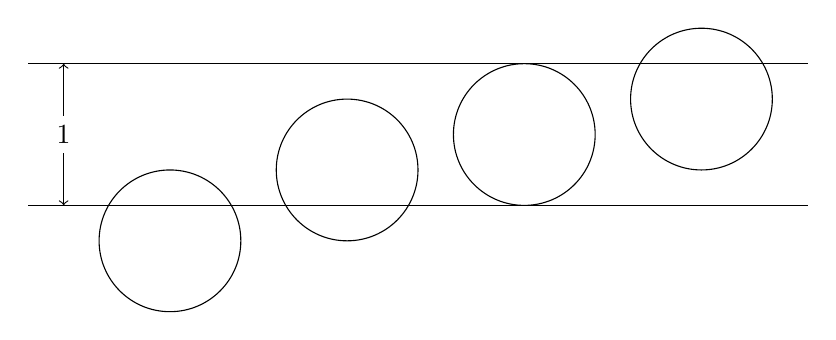
\begin{tikzpicture}[scale=.9]
\draw (0,0) -- (11,0);
\draw (0,2) -- (11,2);
\draw[<->] (.5,0) -- node[fill=white] {$1$} (.5,2);
\foreach \x/\y in {2/-.5, 4.5/.5, 7/1, 9.5/1.5}
  \draw (\x,\y) circle[radius=1];
\end{tikzpicture}
\end{center}
\caption{Solving Buffon's needle with circles}\label{f.buffon3}
\end{figure}

Let $E(a)$ be the expectation of the number of parallel lines crossed by a line of length $a$.

Given a needle of length $a$ we can break it into several segments $\{a_1,\ldots,a_n\}$ and by the linearity of expectation:
\[
E(a) = E\left(\sum_{i=1}^{n} a_i\right) = \sum_{i=1}^{n} E(a_i)\,, 
\]
so it doesn't matter if we compute the expectation of each segment separately. Therefore, if we bend the needle into a circle, the expectation of the number of lines crossed by the circle is the same as the number of lines crossed by the needle.

Consider a line formed into a circle $C$ of \emph{diameter} $1$ and circumference $\pi$. If the circle is thrown onto the surface it will cross lines \emph{exactly} twice (Figure~\ref{f.buffon3}) so:
\begin{equation}\label{eq.buffon-2}
E(C)=2\,.
\end{equation}
Inscribe a regular polygon $Q_n$ (red, dashed) within the circle $C$ (green) and circumscribe a regular polygon $R_n$ (blue, dotted) around $c$ (Figure~\ref{f.buffon4}). Any line that $Q_n$ crosses (red) must also cross the circle and any line that crosses the circle (blue) must also cross $R_n$. Therefore:
\begin{equation}\label{eq.buffon3}
E(Q_n)\leq E(C)\leq E(R_n)\,.
\end{equation}
Let $a_Q, a_R$ be the sums of the lengths of the sides of $Q_n,R_n$, respectively. By the linearity of expectation:
\begin{eqnlabels}\label{eq.buffon1}
E(Q_n)&=&\sum_{i=1}^n E(\textsf{sides of}\;a_Q)=a_QE(1)\\
\label{eq.buffon2}E(R_n)&=&\sum_{i=1}^n E(\textsf{sides of}\;a_R)=a_RE(1)\,. 
\end{eqnlabels}
As $n\rightarrow\infty$ both polygons approximate the circle so:
\begin{equation}\label{eq.buffon-pi}
\lim_{n\rightarrow\infty}a_Q = \lim_{n\rightarrow\infty} a_R=\pi\,,
\end{equation}
the circumference of the circle. From Equations~\ref{eq.buffon1}--\ref{eq.buffon-pi} we have:
\[
\renewcommand*{\arraystretch}{1.5}
\begin{array}{l}
\displaystyle\lim_{n\rightarrow\infty}E(Q_n)=E(C) =\lim_{n\rightarrow\infty}E(R_n)\\
E(C)=aE(1) =\pi E(1) = 2\\
E(1)=\disfrac{2}{\pi}\\
E(a)=aE(1)=\disfrac{2a}{\pi}\,.
\end{array}
\]
\begin{figure}[bt]
\begin{center}
\begin{tikzpicture}
\draw[thick,green!80!black] (0,0) circle[radius=2];
\node[draw,red,thick] (in)
  [minimum size=4cm,regular polygon,regular polygon sides=6]
  at (0,0) {};
\node[draw,blue,rotate=30,thick] (out)
  [minimum size=4.62cm,regular polygon,regular polygon sides=6]
  at (0,0) {};
\node[above left,xshift=5pt] at (in.corner 5) {$Q_n$};
\node[below right,yshift=6pt] at (out.corner 5) {$R_n$};
\draw[thick,red,dashed] (-3,-.6) -- +(6,0);
\draw[very thick,blue,dotted] (-3,1.85) -- +(6,0);
\end{tikzpicture}
\end{center}
\caption{Polygons approximate a circle}\label{f.buffon4}
\end{figure}

\sml{}

Since $\pi=2a/E$ you can obtain an empirical approximation of its value by running the simulation or by throwing needles on a table!

\newpage

\begin{verbatim}
For length = 0.2:
Expectation of crossings = 0.1273
Average crossings        = 0.1308
Empirical value for pi   = 3.0581

For length = 0.5:
Expectation of crossings = 0.3183
Average crossings        = 0.3227
Empirical value for pi   = 3.0989

For length = 1.0:
Expectation of crossings = 0.6366
Average crossings        = 0.6333
Empirical value for pi   = 3.1581
\end{verbatim}

%%%%%%%%%%%%%%%%%%%%%%%%%%%%%%%%%%%%%%%%%%%%%%%%%%%%%%%%%%%%%%%%

\begin{prob}{Buffon's needle with horizontal and vertical rulings}

Solve Buffon's needle problem for a surface that is covered by a grid with squares of size $1\times 1$. A needle can cross a vertical line (green), a horizontal line (blue), both (red) or neither (orange) (Figure~\ref{f.buffon5}).

\begin{figure}[b]
\begin{center}
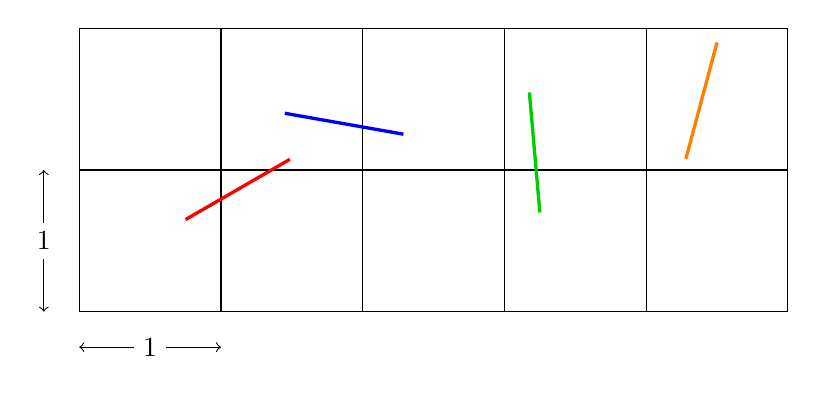
\begin{tikzpicture}[scale=.9]
\draw[step=2cm] (0,0) grid (10,4);
\draw[<->] (-.5,0) -- node[fill=white] {$1$} (-.5,2);
\draw[<->] (0,-.5) -- node[fill=white] {$1$} (2,-.5);
\foreach \x/\y/\a/\c in {
  1.5/1.3/30/red,
  2.9/2.8/-10/blue,
  6.5/1.4/95/green!80!black,
  9/3.8/-105/orange}
    \draw[color=\c,very thick] (\x,\y) -- +(\a:1.7);
\end{tikzpicture}
\end{center}
\caption{Buffon's needle with horizonal and vertical lines}\label{f.buffon5}
\end{figure}

\textbf{Hint:} Are the numbers of crossings of the horizontal and vertical lines independent?

\end{prob}

\solution{}

The numbers of crossings of the horizontal and vertical lines are independent. Let $a$ be the length of a needle. By the linearity of expectation:
\begin{eqn}
E(\textsf{lines crossed by}\; a)&=&E(\textsf{vertical lines crossed by}\; a + \textsf{horizontal lines crossed by}\;a)\\
&=&E(\textsf{vertical lines crossed by}\;a) + E(\textsf{horizontal lines crossed by}\;a)\\
&=&\disfrac{2a}{\pi}+\disfrac{2a}{\pi}=\disfrac{4a}{\pi}\,.
\end{eqn}%
\sml{}

\begin{verbatim}
For length = 0.2:
Expectation of crossings = 0.2546
Average crossings        = 0.2532
For length = 0.5:
Expectation of crossings = 0.6366
Average crossings        = 0.6355
For length = 1.0:
Expectation of crossings = 1.2732
Average crossings        = 1.2736
\end{verbatim}

%%%%%%%%%%%%%%%%%%%%%%%%%%%%%%%%%%%%%%%%%%%%%%%%%%%%%%%%%%%%%%%%

\begin{prob}{Long needles\annotate{D}}

Let the length of the needle in Buffon's problem be $a>1$.

\que{1} What is the expectation of the \emph{number of crossings}?

\que{2} Develop of formula for the probability that there is \emph{at least one crossing}?

\textbf{Hint:} For what angles $\theta$ is the probability a crossing $1$?

\end{prob}

\solution{}

\ans{1} Break the needle into pieces of lengths $\{a_1,a_2,\ldots, a_n\}$, $a_i< 1$, such that $\sum_{i=1}^n a_i=a$. In the solution of Problem~53 we showed that:
\[
E(a)= \sum_{i=1}^n E(a_i)= \disfrac{2a}{\pi}\,.
\]

\ans{2} This solution is based on \cite{wiki-buffon} and \cite[Chapter~26]{proofs}.

By Equation~\ref{eq.cross} the probability that the needle will cross a line is $a\sin\theta$ \emph{if} $a\sin\theta \leq 1$, that is, if $0\leq\theta\leq\sin^{-1}(1/a)$. However, if $a\sin\theta > 1$ then the probability is $1$ (Figure~\ref{f.buffon6}). Generalize Equation~\ref{eq.buffon-integral} for arbitrary $a>0$ by dividing the integral into two parts, one for $\theta\leq\sin^{-1}(1/a))$ and one for $\theta\geq\sin^{-1}(1/a))$:
\begin{eqn}
E(a) &=& \disfrac{2}{\pi}
   \left(\int_{0}^{\sin^{-1}(1/a)} 
   a\sin \theta\:d\theta + 
   \int_{\sin^{-1}(1/a)}^{\pi/2} 1\: d\theta\right)\\
&=& \disfrac{2}{\pi}\left(\left.
    a(-\cos \theta)\right|_0^{\sin^{-1}(1/a)} + 
    \left(\disfrac{\pi}{2} - 
    \sin^{-1}(1/a)\right)\right)\\
&=& 1+\disfrac{2}{\pi}
  \left(a
  \left(1-\sqrt{1-\disfrac{1}{a^2}}\right)-
  \sin^{-1}(1/a)\right)\,.
\end{eqn}%

\begin{figure}[tb]
\begin{center}
\begin{tikzpicture}[scale=1]
\coordinate (O) at (0,0);
\draw (0,0) -- (10,0);
\draw (0,3.5) -- (10,3.5);
\draw[<->] (.5,0) -- node[fill=white,yshift=12pt] {$1$} +(0,3.5);
\draw[<->] (2,0) -- node[fill=white] {$1/2$} +(0,1.75);
\begin{scope}[xshift=0cm,yshift=1.4cm,scale=1]
\coordinate (end1) at (3,-1);
\coordinate (end2) at ($(end1)+(60:3)$);
\coordinate (center) at ($(end1)+(60:1.5)$);
\node[above right,xshift=2pt,yshift=-2pt]
  at (end1) {$\theta$};
\draw[thick] (end1) --  node[left,near end] {$a/2$}
  (center) -- (end2);
\draw[thick] (end2) -- (end2 -| center);
\draw[thick] (end1) -- (end1 -| center);
\draw[thick] (end1 -| center) -- 
  node[right,fill=white,yshift=2pt] {$(a/2)\sin \theta$}
  (center) -- (end2 -| center);
\draw[thick,dotted] (O |- center) -- +(10,0);
\end{scope}
\begin{scope}[xshift=3cm,yshift=.8cm,scale=1.6]
\coordinate (end1) at (2,-1);
\coordinate (end2) at ($(end1)+(60:3)$);
\coordinate (center) at ($(end1)+(60:1.5)$);
\node[above right,xshift=2pt,yshift=-2pt]
  at (end1) {$\theta$};
\draw[thick] (end1) --  node[left,near end] {$a/2$} 
  (center) -- (end2);
\draw[thick] (end2) -- (end2 -| center);
\draw[thick] (end1) -- (end1 -| center);
\draw[thick] (end1 -| center) -- 
  node[right,fill=white,yshift=6pt] {$(a/2)\sin \theta$}
  (center) -- (end2 -| center);
\end{scope}
\end{tikzpicture}
\end{center}
\caption{Long needles}\label{f.buffon6}
\end{figure}

\sml{}
\begin{verbatim}
For length = 1.5:
Expectation of crossings = 0.7786
Average crossings        = 0.7780
For length = 2.0:
Expectation of crossings = 0.8372
Average crossings        = 0.8383
For length = 3.0:
Expectation of crossings = 0.8929
Average crossings        = 0.8897
\end{verbatim}

%%%%%%%%%%%%%%%%%%%%%%%%%%%%%%%%%%%%%%%%%%%%%%%%%%%%%%%%%%%%%%%%

\newpage

\begin{prob}{Molina's urns}
Let $U_1,U_2$ be two urns. $U_1$ has $w_1$ white balls and $b_1$ black balls, while $U_2$ has $w_2$ white balls and $b_2$ black balls. It is given that $w_1+b_1=w_2+b_2$. $n$ balls are drawn \emph{with replacement} from each urn. For various values of $n>1$ find $w_1,b_1,w_2,b_2$ such that:
\[
P(\textsf{balls drawn from} \;U_1\; \textsf{are all white})=
P(\textsf{balls drawn from} \;U_2\; \textsf{are all white or all black})\,.
\]
\vspace{-6ex}
\end{prob}

\solution{}

For $n=2$ the equation that must be solved is:
\begin{eqn}
\left(\disfrac{w_1}{m}\right)^2&=&\left(\disfrac{w_2}{m}\right)^2+\left(\disfrac{b_2}{m}\right)^2\\
w_1^2&=&w_2^2+b_2^2\,,
\end{eqn}%
and any Pythagorean triple is a solution.

By Fermat's Last Theorem, proved in $1995$ by Andrew Wiles, there are no solutions to $w_1^n=w_2^n+b_2^n$ for $n\geq 3$.

\sml{}

The simulation was run for $n=2$ and several Pythagorean triples.
\begin{verbatim}
For w1 = 17, w2 = 8, b2 =15:
Proportion of two whites in urn 1          = 0.5523
Proportion of two whites or black in urn 2 = 0.5387
For w1 = 29, w2 = 20, b2 =21:
Proportion of two whites in urn 1          = 0.5003
Proportion of two whites or black in urn 2 = 0.5026
For w1 = 65, w2 = 33, b2 =56:
Proportion of two whites in urn 1          = 0.5381
Proportion of two whites or black in urn 2 = 0.5384
\end{verbatim}

%%%%%%%%%%%%%%%%%%%%%%%%%%%%%%%%%%%%%%%%%%%%%%%%%%%%%%%%%%%%%%%%
